\documentclass{article}
\usepackage{graphicx}

\title{\textbf{2025 Parallel and Distributed Computing Assignment \#1}}
\date{April 4, 2025}
\author{Doyoung Kim}

\begin{document}
\maketitle
In this assignment, we are aimed to write a parallel program that performs LU
decomposition using OpenMP. OpenMP allows programmers to write portable 
concurrent programs without caring about the platform-specific behaviours. Also,
using OpenMP, programmers can write unified code for the sequential version of
the program and the parallel version of the program. 

LU decomposition is a procedure that decomposes a given matrix into two matrix,
namely $L$ and $R$. The relationship between the target matrix $A$ and the
decomposition results is given as follows, where $P$ stands for the permutation
matrix.

$$PA=LU$$

One of algorithms for LU decomposition is LU decomposition with partial 
pivoting. This algorithm picks the greatest value at each column, and treat the
value as pivot. Then, it swaps the row that contains the pivot with the first
row in current block. A concrete description about the algorithm was introduced
in the assignment handout, so this report will not further explain about the
algorithm.

\section{Implementation}
One notable point of the program is that a square matrix is represented as a 
linear, contiguous array with the size of $N^2$. This is to utilize cache
locality as much as possible. If it were implemented as a \verb|std::vector| of 
\verb|std::vector|s or array of arrays, the rows may be stored in different
blocks of heap, making it hard to take advantage of the locality of the cache.

The main routine of this program is \verb|run()| function, which performs the
decomposition using the algorithm mentioned above. While the serial version 
directly applies the row pivoting algorithm, the parallel version of the program
creates a team of thread at the beginning of the top-level loop. These threads
share the decomposed matrix and the target matrices, along with the permutation
vector and size of the matrices. One might argue that this may cause data races
among the threads. However, this is not true since each element is 'owned' by
one thread, eliminating the possibility of data races.

Another point that is worth mentioning is that the top-level loop itself, which
iterates on the size of remaining block(\verb|k|) is not parallelized since 
this iteration must be done sequentially. Since the result of a previous 
iteration is used in the current iterative step, the threads must join after
each execution of the top-level iterations. In other words, the threads should
be synchronized after the top-level loop.

Inner loops that iterates on each element, or row are where the parallelism is
actually utilized. First, the program let those threads to find the pivot row 
parallelly. Second, each thread calculates the element of the target matrices
- \verb|l| and \verb|u| - assigned to it. Lastly, each thread performs 
subtraction on each element of matrix \verb|a|.

\section{Efficiency}
The running times are measured by \verb|std::chrono::steady_clock|. The time to 
generate input matrix and initialize output matrices was not included to this 
measure. The testing machine was MacBook Pro M3, 11 core model with an 
integrated memory of 18 GiB. The program was run on a Docker container with
Ubuntu 24.04 image. The program was executed 5 times, and the result shown in 
below figures are the average of them.

\begin{figure}[h]
\centering
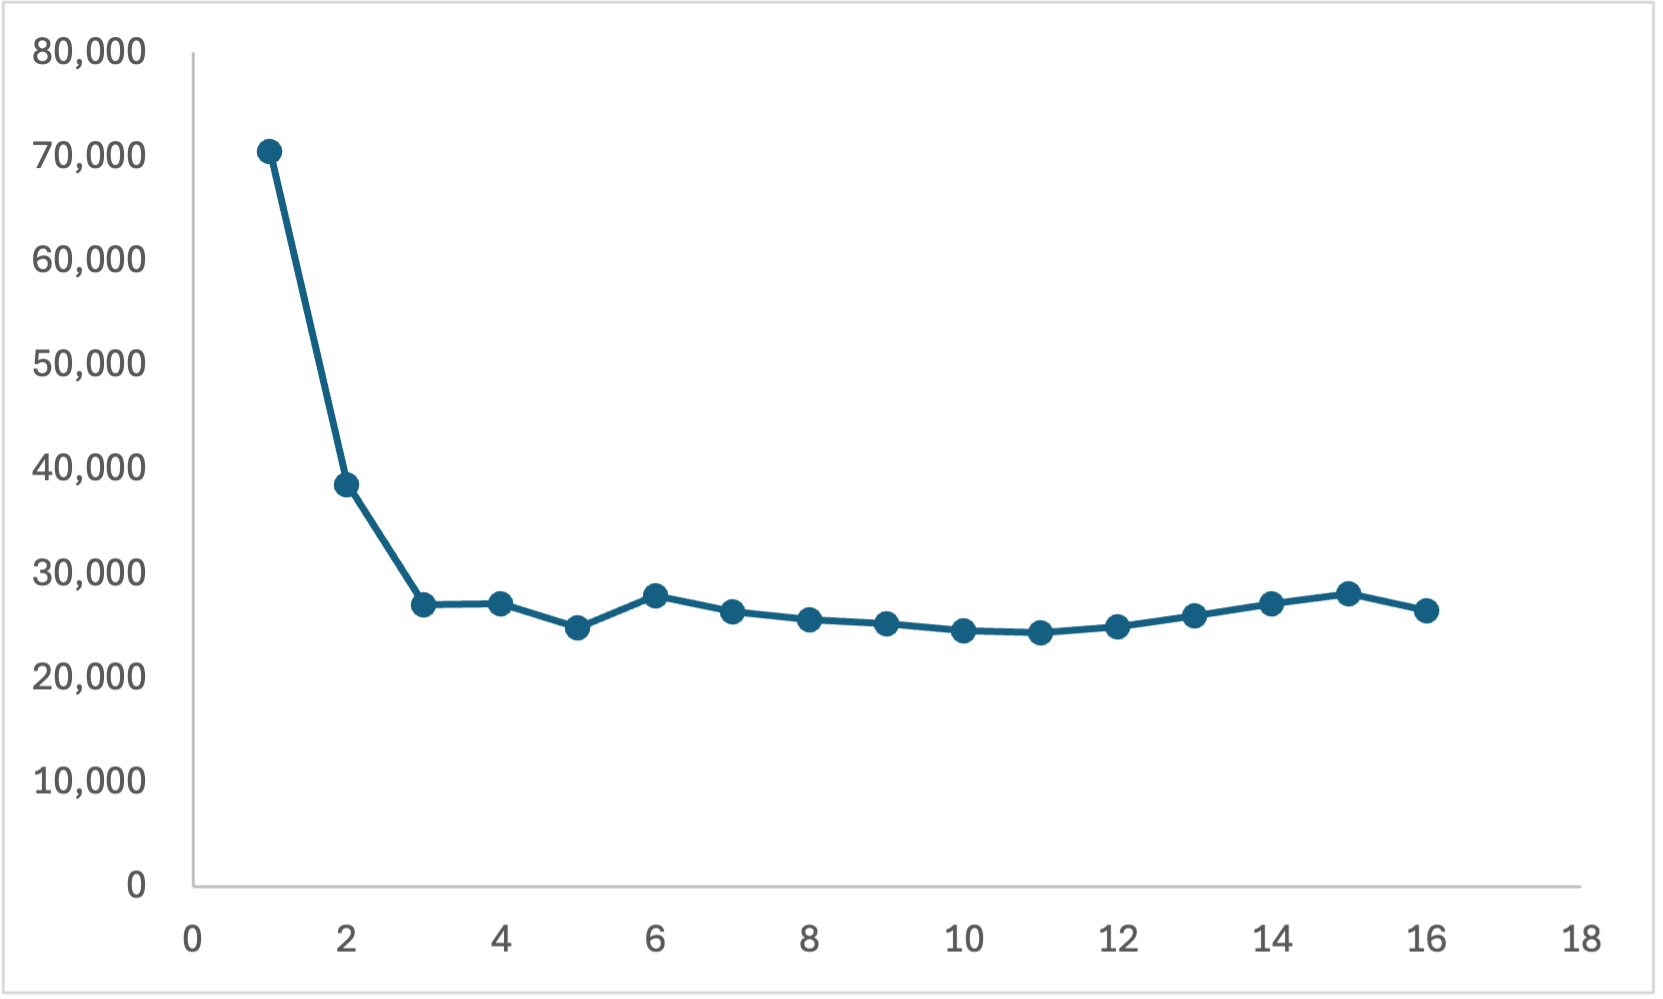
\includegraphics[width=.75\textwidth]{figure1.png}
\caption{
    Plot of running time according to the number of threads. The X-axis shows 
    the number of threads, while the Y-axis represents the running time, 
    measured in milliseconds. The time for single thread execution was measured
    with serial binary. 
}
\end{figure}

Figure 1 shows the measured running time versus the number of threads. As one
can expect, the running time decreases rapidly as the number of threads 
increases to a certain point. However, this tendency does not maintained for
more than 3 threads. 

\begin{figure}[h]
\centering
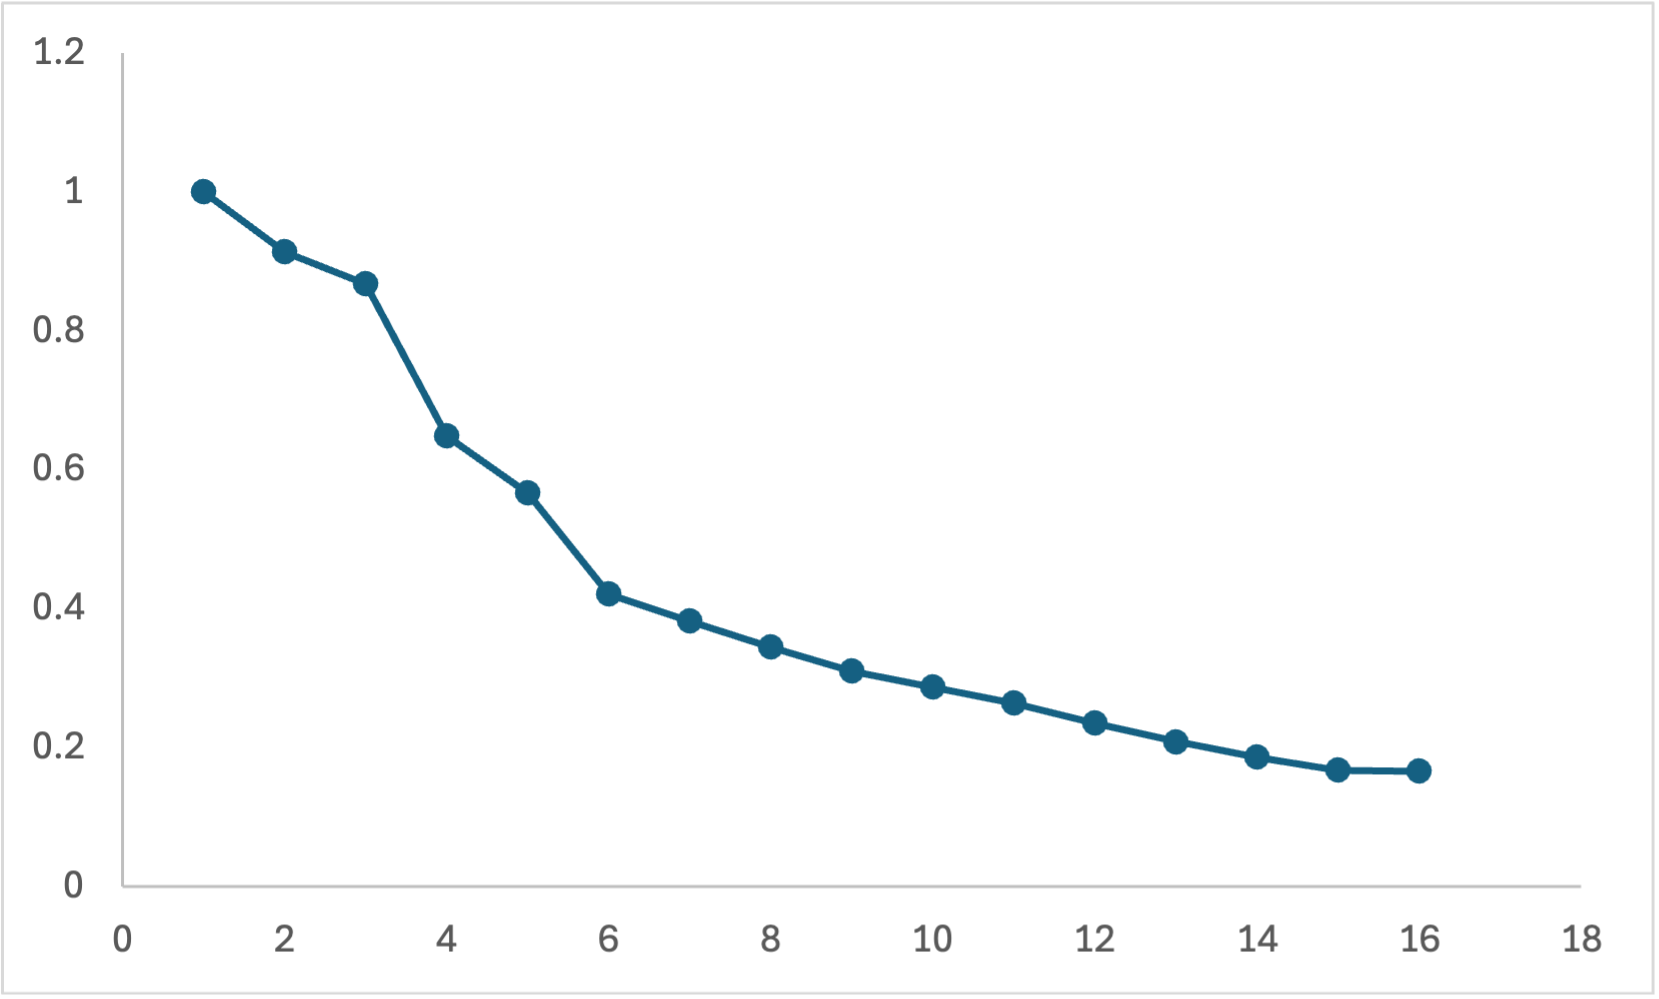
\includegraphics[width=.75\textwidth]{figure2.png}
\caption{
    Plot of parallel efficiency according to the number of threads. The X-axis 
    shows the number of threads, while the Y-axis represents the parallel 
    efficiency, calculated as $\frac{S}{pT(p)}$ where $S$ stands for
    the serial execution time, $p$ for the number of threads, $T(p)$ for the
    measured parallel execution time for $p$.
}
\end{figure}

Figure 2 shows the parallel efficiency derived by the execution time for each
number of threads. Since the execution time does not decrease after the thread
number of 3, we can observe the parallel efficiency proportionally decreasing
after this point.

One explanation for this phenomenon is that there are inherent sequential 
dependency for each loop. In current implementation, threads must await the
execution of other threads since each inner for loop depends on the result
of the previous one. Due to this sequential dependency, the parallel execution
time is limited to certain point, resulting in decrease in the parallel 
efficiency.

\section{Conclusion}
In this assignment, we have implemented a parallel algorithm using OpenMP 
library, and measured the wall clock time for the execution of the program. 
Also, we have observed the changes in the execution time, providing different
thread number as an argument. This performance evaluation demonstrated that 
assigning more threads to the program does not always result in smaller 
execution time due to a sequential bottleneck. 

One possible improvement for current implementation is to use directives such
as \verb|nowait| to allow threads to process next task. Since threads have to
pause its execution until the other threads are done in their job, there is
some lost performance boost opportunities. Nonetheless, this requires careful
analysis on data dependency between each inner loops.

\end{document}